% 编译使用xelatex编译一次

\documentclass[12pt, a4paper, oneside]{ctexart}
\usepackage{subcaption,listings,amsmath, amsthm, amssymb, bm, color, framed,float, graphicx, hyperref, mathrsfs,minipage-marginpar}

\title{\textbf{数据库系统作业三}}
\author{2021113140符世博}
\date{}
\linespread{1.5}
\definecolor{shadecolor}{RGB}{241, 241, 255}
\newcounter{problemname}
\newenvironment{problem}{\begin{shaded}\stepcounter{problemname}\par\noindent\textbf{题目\arabic{problemname}. }}{\end{shaded}\par}
\newenvironment{solution}{\par\noindent\textbf{解答. }}{\par}
\newenvironment{note}{\par\noindent\textbf{题目\arabic{problemname}的注记. }}{\par}


\begin{document}
    \maketitle
    
    \begin{problem}
        在图书管理数据库中,有如下三个关系:

        图书信息关系:B(B\#, BNAME, AUTHOR, TYPE),其中B\#为图书编号,BNAME为书名,
        AUTHOR为作者,TYPE为类别;

        学生信息关系:S(S\#, SNAME, CLASS),其中S\#为学号,SNAME为学生姓名,CLASS为班级
        号;

        借阅信息关系:L(S\#, B\#, DATE),其中S\#为借阅人学号,B\#为被借阅图书编号,DATE为借阅日
        期。

        使用SQL语言回答以下问题:

        (1)删除“《西游记》”这本书的所有借阅信息

        (2)查询“201”班学生借阅图书的书名

        (3)查询“小明”借过,但“小李”没有借过的图书的编号

        (4)查询被借阅过的每本书的图书编号和借阅次数
    \end{problem}
    \begin{solution}
        \par
        (1)
        
        DELETE FROM L

        WHERE B\# IN(

        SELECT B\#

        FROM B

        WHERE BNAME=“西游记”

        );

        (2)
        
        SELECT B.BNAME

        
        FROM B
        
        JOIN L ON B.B\# = L.B\#
        
        JOIN S ON S.S\# = L.S\#
        
        WHERE S.CLASS = “201”;

        (3)
        
        SELECT L.B\#

        FROM L

        JOIN S ON S.S\# = L.S\#

        WHERE S.SNAME = '小明'

        AND L.B\# NOT IN (

        SELECT L.B\#

        FROM L

        JOIN S ON S.S\# = L.S\#

        WHERE S.SNAME = '小李'

        );

        (4)

        SELECT L.B\#,COUNT(*) AS BorrowCount

        FROM L

        GROUP BY L.B\#;

    \end{solution}

    \begin{problem}
        在学生成绩数据库中,有如下三个关系:

        学生信息关系:S(S\#, SNAME, D\#),其中S\#为学号,SNAME为学生姓名,D\#为所在系名;

        学生成绩关系:SC(S\#, C\#, Grade),其中S\#为学号,C\#为课程号,Grade为成绩;

        系信息关系:D(D\#, Addr),其中D\#为系名,Addr为所在地址

        使用SQL语言回答以下问题:

        (1)查询“物理系”的全体学,按学号升序排列

        (2)查询姓王的学生的学号姓名

        (3)定义一个视图 SumC(S\#, SNAME, Count), 其中 S\#为学号, SNAME 为学生姓名, Count
        为该学生的选课课程个数

        (4)查询既选修了“1002”课程的学生中选修了“1003”课程的学生姓名
    \end{problem}
    \begin{solution}
        \par
        (1)

        SELECT S\#

        FROM S

        WHERE D\#=“物理系”

        ORDER BY S\# ASC;
        
        (2)

        SELECT S\#,SNAME
        
        FROM S
        
        WHERE SNAME LIKE “王\%”;

        (3)

        CREATE VIEW SumC AS

        SELECT S.S\#,S.SNAME,COUNT(SC.C\#) AS CounT

        FROM S
        
        LEFT JOIN SC ON S.S\#=SC.S\#
        
        GROUP BY S.SNAME

        (4)

        SELECT S.SNAME

        FROME S

        JOIN SC SC1 ON S.S\#=SC1.S\#

        JOIN SC SC2 ON S.S\#=SC2.S\#

        WHERE SC1.C\#=“1002” AND SC2.C\#=“1003”;

    \end{solution}

    \begin{problem}
        在第 2 题学生成绩数据库中, 若 S 关系中有学生选课, 则 SC 关系中有该学生的 S\#和C\#记录, 否则没有, 则使用 SQL 语言回答以下问题:

        (1)查询选过课的学生的学号和姓名

        (2)查询没选过课的学生的学号和姓名
    \end{problem}
    \begin{solution}
        \par
        (1)

        SELECT S.S\#,S.SNAME
        
        FROM S
        
        JOIN SC ON S.S\#=SC.S\#
        
        GROUP BY S.S\#,S.SNAME

        (2)

        SELECT S.S\#,S.SNAME

        FROM S

        LEFT JOIN SC ON S.S\#=SC.S\#

        WHERE SC.S\# IS NULL;

    \end{solution}
    \begin{problem}
        设有如下实体:
        科研人员: 职工号、 姓名、 性别、 年龄、 专业、 研究方向、 所在办公室
        科研项目: 研究项目编号、 项目名称、 项目经费、 项目负责人
        办公室: 房间编号、 面积、 办公电话
        上述实体存在如下联系:
        \begin{enumerate}
            \item 一个科研项目可以有多名研究人员参加, 一个研究人员也可以参加多个研究项目
            \item 每个项目由一个科研人员担任负责人
            \item 一个办公室可以有多个科研人员办公, 而一个科研人员只能在一个办公室里办公
        \end{enumerate}
        设计该系统的 ER 图, 并写出对应的关系模式, 标明主键
    \end{problem}
    \begin{solution}
        \begin{figure}[H]
            \centering
            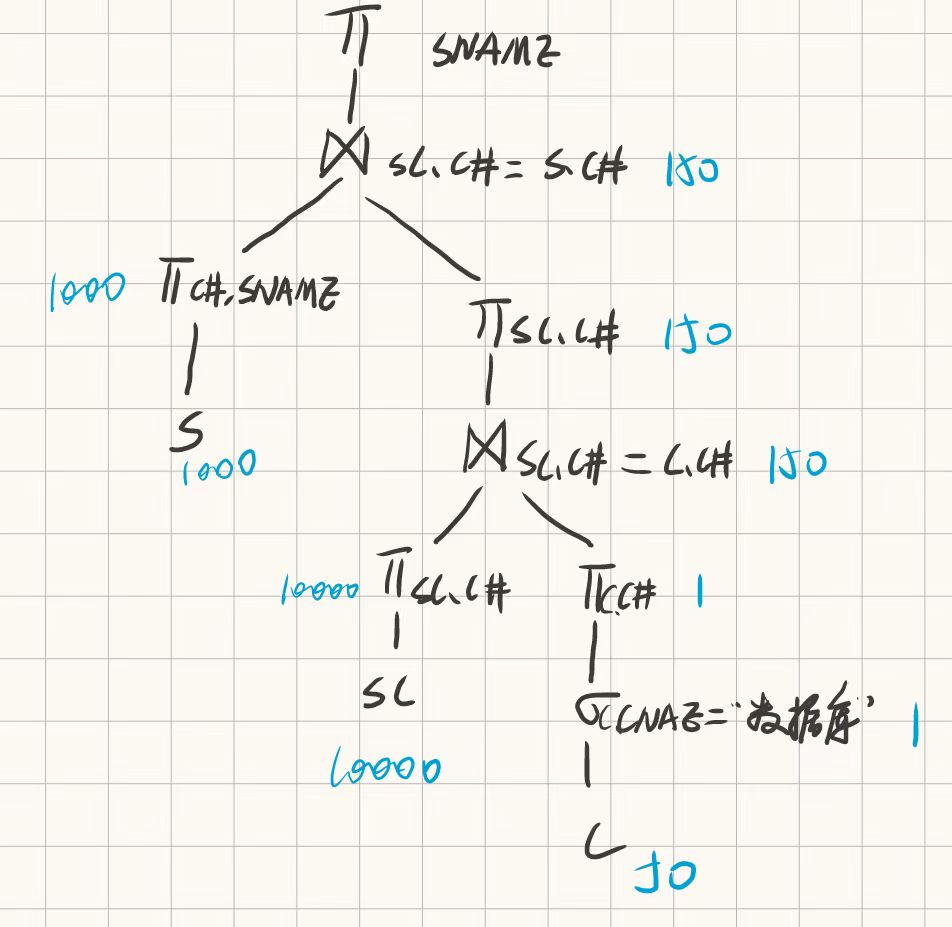
\includegraphics[width=0.95\textwidth]{img/4.jpg}
        \end{figure}
    \end{solution}
    \begin{problem}
        设有如下实体:
        单位: 单位名、 电话
        职工: 职工号、 姓名、 性别
        设备: 设备号、 设备名、 产地
        供应商: 姓名、 电话
        工程: 工程名、 地名
        上述实体存在如下联系:
        \begin{enumerate}
            \item 一个单位有多个职工, 一个职工只隶属于一个单位
            \item 一个职工只参与一个工程, 一个工程中有多个职工参加工作
            \item 有多个供应商为各个工程供应不同的设备
        \end{enumerate}
        试完成如下工作:
        \begin{enumerate}
            \item 设计该 E-R 图
            \item 将该 E-R 图转换为等价的关系模式表示的数据库逻辑结构
        \end{enumerate} 
    \end{problem}
    \begin{solution}
        (1)
        \begin{figure}[H]
            \centering
            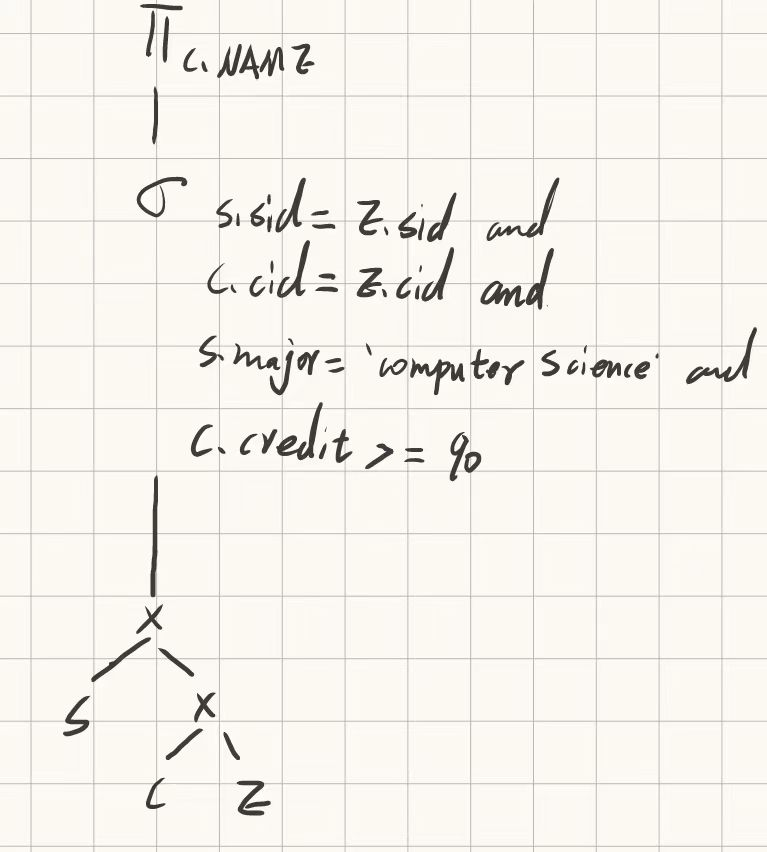
\includegraphics[width=0.95\textwidth]{img/5.jpg}
        \end{figure}
        (2)
        
        单位(单位名,电话)

        职工(职工号,姓名,性别)

        工程(工程名,地名)

        供应商(姓名,电话)

        设备(设备号,设备名,产地)

        隶属(单位名,职工号)

        参与(工程名,职工号)

        供应(姓名,工程名,设备号)

    \end{solution}

\end{document}